\documentclass{article}
\usepackage[utf8x]{inputenc}
\usepackage{ucs}
\usepackage{amsmath} 
\usepackage{amsfonts}
\usepackage{upgreek}
\usepackage[english,russian]{babel}
\usepackage{graphicx}
\usepackage{float}
\usepackage{textcomp}
\usepackage{hyperref}
\usepackage{geometry}
  \geometry{left=2cm}
  \geometry{right=1.5cm}
  \geometry{top=1cm}
  \geometry{bottom=2cm}
\usepackage{tikz}
\usepackage{ccaption}
\usepackage{multicol}

\usepackage{listings}
%\setlength{\columnsep}{1.5cm}
%\setlength{\columnseprule}{0.2pt}


\begin{document}
\pagenumbering{gobble}

\lstset{
  language=C,                % choose the language of the code
  basicstyle=\linespread{1.1}\ttfamily,
  columns=fixed,
  fontadjust=true,
  basewidth=0.5em,
  keywordstyle=\color{blue}\bfseries,
  commentstyle=\color{gray},
  stringstyle=\ttfamily\color{orange!50!black},
  showstringspaces=false,
  %numbers=false,                   % where to put the line-numbers
  numbersep=5pt,
  numberstyle=\tiny\color{black},
  numberfirstline=true,
  stepnumber=1,                   % the step between two line-numbers.        
  numbersep=10pt,                  % how far the line-numbers are from the code
  backgroundcolor=\color{white},  % choose the background color. You must add \usepackage{color}
  showstringspaces=false,         % underline spaces within strings
  captionpos=b,                   % sets the caption-position to bottom
  breaklines=true,                % sets automatic line breaking
  breakatwhitespace=true,         % sets if automatic breaks should only happen at whitespace
  xleftmargin=.2in,
  extendedchars=\true,
  keepspaces = true,
}
\lstset{literate=%
   *{0}{{{\color{red!20!violet}0}}}1
    {1}{{{\color{red!20!violet}1}}}1
    {2}{{{\color{red!20!violet}2}}}1
    {3}{{{\color{red!20!violet}3}}}1
    {4}{{{\color{red!20!violet}4}}}1
    {5}{{{\color{red!20!violet}5}}}1
    {6}{{{\color{red!20!violet}6}}}1
    {7}{{{\color{red!20!violet}7}}}1
    {8}{{{\color{red!20!violet}8}}}1
    {9}{{{\color{red!20!violet}9}}}1
}

\section*{Домашнее задание №1}
Материалы по этому заданию доступны по ссылке: \href{https://github.com/v-biryukov/cs_mipt_faki/tree/master/term2}{https://github.com/v-biryukov/cs\_mipt\_faki/tree/master/term2}\\
Для компиляции используйте компилятор g++ на Linux/MacOs или компилятор MinGW на Windows.

\subsection*{Класс Quaternion}
В папке \texttt{classes/Complex} лежит реализация класса комплексных чисел. Подлючите файл \texttt{complex.h} к вашей программе и выполните следующее:
\begin{enumerate}
\item Создайте комплексное число $5+4i$, разделите его на $i$ и напечатайте.
\item Создайте комплексное число $z = \frac{1+i}{\sqrt{2}}$, найдите чему равно $z^8$ и напечатайте.
\item Написать функцию \texttt{Complex sin(Complex z)}, которая вычисляет синус комплексного числа.
\item Создайте вектор комплесных чисел, заполните его 5-ю произвольными комплексными числами. Найдите сумму этих комплексных чисел двумя разными способами:
	\begin{enumerate}
	\item С помощью цикла \texttt{for}. Используйте итератор \texttt{std::vector<Complex>::iterator}.
	\item С помощью функции \texttt{std::accumulate()} из библиотеки \texttt{numeric}.
	\end{enumerate}
\end{enumerate}
\subsection*{Класс Image}
В папке \texttt{classes/Image} лежит реализация класса изображений. Подлючите файл \texttt{image.h} к вашей программе.
\begin{figure}[H]
\center{
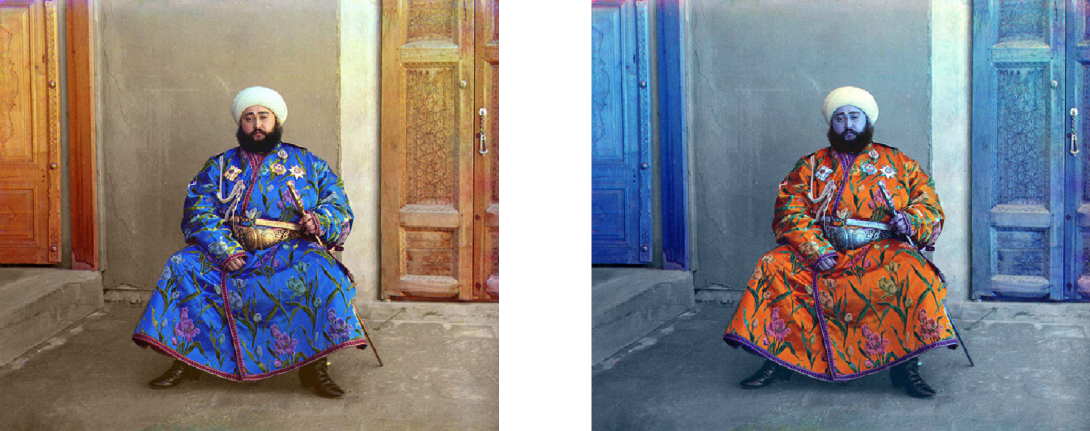
\includegraphics[width=0.7\linewidth]{image_example.png}\\
Рисунок 1: Пример обработки изображения с помощью класса Image
}
\end{figure}

\begin{enumerate}
\item \textbf{Компиляция:} Скомпилируйте файлы \texttt{image.cpp} и \texttt{main.cpp} в папке \texttt{classes/Image}. При компиляции вам нужно указать оба исполняемых файла: \texttt{g++ image.cpp main.cpp}. Запустите и посмотрите на результат работы программы.
\item \textbf{Black and White:} Добавьте метод \texttt{void blackwhite()} к классу \texttt{Image}, который будет делать изображение черно-белым. Подсказка: у черно-белого изображения все компоненты цвета равны.
\item \textbf{*Свёртка:} Добавьте метод \texttt{void convolve(int n, int m, float filter[])} к классу \texttt{Image}, который будет делать свёртку изображения с фильтром(другое название -- ядро). \texttt{filter} это массив размера $n \times m$. Пиксель нового изображения с координатами x, y определяется следующим образом: 
$$B[x][y] = \sum_{i=0}^{n-1} \sum_{j=0}^{m-1} A[x+i-n/2][y+j-m/2]*f[i][j]$$
, где $A$ -- старое изображение, $B$ -- новое, $f$ -- массив filter. При выходе за границы массива $A$ берем в качестве значений нули. \\
По следующей ссылке можно найти примеры обработки изображения с помощью различных матричных фильтров
\href{https://en.wikipedia.org/wiki/Kernel_(image_processing)}{https://en.wikipedia.org/wiki/Kernel\_(image\_processing)}
Добавьте методы \texttt{blur()}, \texttt{edges()} и \texttt{sharpen()} к классу \texttt{Image} которые будут вызывать метод \texttt{convolve} с различными фильтрами. Протестировать эти методы на различных изображениях.\\
Более подробно об операции свёртки:
\href{https://www.youtube.com/watch?v=X5O6wVmOYvk}{https://www.youtube.com/watch?v=X5O6wVmOYvk}


\item \textbf{Задача об убегающей точке:} Предположим, что у нас есть комплексная функция $f(z) = z^2$. Выберем некоторое комплексное число $z_0$ и будем проводить следующие итерации: $z_1 = f(z_0), z_2 = f(z_1), ..., z_{n+1} = f(z_n)$. В зависимости от выбора точки $z_0$ эта последовательность либо разойдётся, либо останется в некоторой ограниченной области. Нужно найти все точки комплексной плоскости, которые не являются убегающими. \\
Для функции $f(z) = z^2$ эта область тривиальна, но всё становится сложней для функции вида $f(z) = z^2 + c$, где $c$ -- некоторое комплексное число. Численно найдите область убегания для функций такого вида. Для этого создайте изображение размера 1000x1000, покрывающую область [-2:2]x[-2:2] на комплексной плоскости. Для каждой точки этой плоскости проведите $N=50$ итераций и, в зависимости от результата, окрасьте пиксель в соответствующий цвет (цвет можно подобрать самим). Используйте классы Complex и Image. Программа должна создавать файл \texttt{juliaset.ppm}.\\
Добавьте параметры командной строки: 2 вещественных числа, соответствующие комплексному числу c, и целое число итераций $N$. 

\item \textbf{Множество:} Зафиксируем теперь $z_0 = 0$ и будем менять $c$. Численно найдите все параметры $c$, для которых точка не является убегающей. Программа должна создавать файл \texttt{mandelbset.ppm}.


\item \textbf{Волновой алгоритм поиска пути:} В папке \texttt{wave\_algo\_tests} лежат ppm изображения. Задача -- по картинке построить кратчайший путь от начала(зелёный пиксель) до конца(красный пиксель) ходить можно только по белым пикселям. Путь нужно нарисовать на картинке, а новую картинку сохранить.
\end{enumerate}
\end{document}